\achapter{24}{Orthogonal and Orthonormal Bases in $\R^n$} \label{chap:orthogonal_basis}

\vspace*{-17 pt}
\framebox{
\parbox{\dimexpr\linewidth-3\fboxsep-3\fboxrule}
{\begin{fqs}
\item What is an orthogonal set in $\R^n$? What is one useful fact about orthogonal subsets of $\R^n$? 
\item What is an orthogonal basis for a subspace of $\R^n$? What is an orthonormal basis?
\item How does orthogonality help us find the weights to write a vector as a linear combination of vectors in an orthogonal basis?  
\item What is an orthogonal matrix and why are orthogonal matrices useful? 
%\item How can we find a least squares solution to an equation $A \vx = \vb$? 
\end{fqs}}}%\hspace*{3 pt}}

\vspace*{13 pt}

\csection{Application: Rotations in 3D} 
\label{sec:appl_3d_rotate}

An aircraft in flight, like a plane or the space shuttle, can perform three independent rotations: \emph{roll}, \emph{pitch}, and \emph{yaw}. Roll is a rotation about the axis through the nose and tail of the aircraft, pitch is rotation moving the nose of the aircraft up or down through the axis from wingtip to wingtip, and yaw is the rotation when the nose of the aircraft turns left or right about the axis though the plane from top to bottom. These rotations take place in $3$-space and the axes of the rotations change as the aircraft travels through space. To understand how aircraft maneuver, it is important to know about general rotations in space. These are more complicated than rotations in $2$-space, and, as we will see later in this section, involve orthogonal sets. 

\csection{Introduction}
\label{sec:orthog_set_intro}

If $\CB = \{\vv_1, \vv_2, \ldots, \vv_m\}$ is a basis for a subspace $W$ of $\R^n$, we know that any vector $\vw$ in $W$ can be written uniquely as a linear combination of the vectors in $\CB$. In the past, the way we have found the coordinates of $\vx$ with respect to $\CB$, i.e. the weights needed to write a vector $\vx$ as a linear combination of the elements in $\CB$, has been to row reduce the matrix $[\vv_1  \ \vv_2  \ \cdots  \ \vv_m \ | \ \vx]$ to solve the corresponding system. This can be a cumbersome process, especially if we need to do it many times. This process also forces us to determine all of the weights at once. For certain types of bases, namely the \emph{orthogonal} and \emph{orthonormal} bases, there is a much easier way to find individual weights for this linear combination.

Recall that two nonzero vectors $\vu$ and $\vv$ in $\R^n$ are orthogonal if $\vu \cdot \vv = 0$. We can extend this idea to an entire set. For example, the standard basis $\CS = \{\ve_1, \ve_2, \ve_3\}$ for $\R^3$ has the property that any two distinct vectors in $\CS$ are orthogonal to each other. The basis vectors in $\CS$ make a very nice coordinate system for $\R^3$, where the basis vectors provide the directions for the coordinate axes. We could rotate this standard basis, or multiply any of the vectors in the basis by a nonzero constant, and retain a basis in which all distinct vectors are orthogonal to each other (e.g., $\{[2 \ 0 \ 0]^{\tr}, [0 \ 3 \ 0]^{\tr}, [0 \ 0 \ 1]^{\tr}\}$). We define this idea of having all vectors be orthogonal to each other for sets, and then for bases.

\begin{definition} \label{def:6_b_orthogonal_set_Rn} A non-empty subset $S$ of $\R^n$ is \textbf{orthogonal}\index{orthogonal set in $\R^n$} if $\vu \cdot \vv = 0$ for every pair of distinct vectors $\vu$ and $\vv$ in $S$.
\end{definition}

\begin{pa} \label{pa:6_b} ~
\be
\item Determine if the set $S = \{[1 \ 2 \ 1]^{\tr}, [2 \ -1 \ 0]^{\tr}\}$ is an orthogonal set.


\item Orthogonal bases are especially important.

\begin{definition} \label{def:6_b_orthogonal_basis_Rn} An \textbf{orthogonal basis}\index{orthogonal basis in $\R^n$} $\CB$ for a subspace $W$ of $\R^n$ is a basis of $W$ that is also an orthogonal set.
\end{definition}

Let $\CB = \{\vv_1, \vv_2, \vv_3\}$, where $\vv_1 = [1 \ 2 \ 1]^{\tr}$, $\vv_2 = [2 \ -1 \ 0]^{\tr}$, and $\vv_3 = [1 \ 2 \ -5]^{\tr}$. 
    \ba
    \item Explain why $\CB$ is an orthogonal basis for $\R^3$.


    \item Suppose $\vx$ has coordinates $x_1, x_2, x_3$ with respect to the basis $\CB$, i.e. 
\[ \vx = x_1 \vv_1 + x_2 \vv_2 + x_3 \vv_3 \,.\]
Substitute this expression for $\vx$ in $\vx \cdot \vv_1$ and use the orthogonality property of the basis $\CB$ to show that $x_1 = \frac{\vx \cdot \vv_1}{\vv_1 \cdot \vv_1}$. Then determine $x_2$ and $x_3$ similarly. Finally, calculate the values of $x_1$, $x_2$, and $x_3$ if $\vx = [1 \ 1 \ 1]^{\tr}$. 


   \item Find components of $\vx = [1 \ 1 \ 1]^{\tr}$ by reducing the augmented matrix $[\vv_1 \   \vv_2 \  \vv_3 \ | \ \vx]$. Does this result agree with your work from the previous part?

    \ea

\ee

\end{pa}

\csection{Orthogonal Sets}
\label{sec:orthog_sets}

We defined orthogonal sets in $\R^n$ and bases of subspaces of $\R^n$ in Definitions \ref{def:6_b_orthogonal_set_Rn} and \ref{def:6_b_orthogonal_basis_Rn}. We saw that the standard basis in $\R^3$ is an orthogonal set and an orthogonal basis of $\R^3$ -- there are many other examples as well.



\begin{activity} \label{act:6_b_orthog} Let $\vw_1 = \left[ \begin{array}{r} -2 \\ 1 \\ -1 \end{array} \right]$, $\vw_2 = \left[ \begin{array}{r} 0 \\ 1 \\ 1 \end{array} \right]$, and $\vw_3 = \left[ \begin{array}{r} 1 \\ 1 \\ -1 \end{array} \right]$. In the same manner as in Preview Activity \ref{pa:6_b}, we can show that the set $S_1 = \left\{ \vw_1, \vw_2, \vw_3  \right\}$ is an orthogonal subset of $\R^3$. 
	\ba
	\item Is the set $S_2 = \left\{ \left[ \begin{array}{r} -2 \\ 1 \\ -1 \end{array} \right], \left[ \begin{array}{r} 0 \\ 1 \\ 1 \end{array} \right], \left[ \begin{array}{r} 1 \\ 1 \\ -1 \end{array} \right], \left[ \begin{array}{r} 1 \\ 2 \\ 0 \end{array} \right] \right\}$ an orthogonal subset of $\R^3$?
	
	

	\item Suppose a vector $\vv$ is a vector so that $S_1 \cup \{\vv\}$ is an orthogonal subset of $\R^3$. Then $\vw_i \cdot \vv = 0$ for each $i$. Explain why this implies that $\vv$ is in $\Nul A$, where $A =  \left[ \begin{array}{rcr} -2&1&-1 \\ 0&1&1 \\ 1&1&-1 \end{array} \right]$. 
	
	\item Assuming that the reduced row echelon form of the matrix $A$ is $I_3$, explain why it is not possible to find a nonzero vector $\vv$ so that $S_1 \cup \{\vv\}$ is an orthogonal subset of $\R^3$. 
		

	
	\ea
\end{activity}


The example from Activity \ref{act:6_b_orthog} suggests that we can have three orthogonal nonzero vectors in $\R^3$, but no more. Orthogonal vectors are, in a sense, as far apart as they can be. So we might expect that there is no linear relationship between orthogonal vectors. The following theorem makes this clear.

\begin{theorem} \label{thm:6_b_Orth_li} Let $\{\vv_1, \vv_2, \ldots, \vv_m\}$ be a set of nonzero orthogonal vectors in $\R^n$. Then the vectors $\vv_1, \vv_2, \ldots, \vv_m$ are linearly independent.
\end{theorem}

\begin{proof} Let $S = \{\vv_1, \vv_2, \ldots, \vv_m\}$ be a set of nonzero orthogonal vectors in $\R^n$. To show that $\vv_1$, $\vv_2$, $\ldots$, $\vv_m$ are linearly independent, assume that
\begin{equation}
x_1\vv_1 + x_2\vv_2 + \cdots + x_m \vv_m = \vzero \label{eq:6_b_orthog}
\end{equation}
for some scalars $x_1$, $x_2$, $\ldots$, $x_m$. We will show that $x_i = 0$ for each $i$ from 1 to $m$. Since the vectors in $S$ are orthogonal  to each other, we know that $\vv_i \cdot \vv_j = 0$ whenever $i \neq j$. Fix an index $k$ between 1 and $m$. We evaluate the dot product of both sides of (\ref{eq:6_b_orthog}) with $\vv_k$ and simplify using the dot product properties:
\begin{align}
\vv_k \cdot (x_1\vv_1 + x_2\vv_2 + \cdots + x_m \vv_m) &= \vv_k \cdot \vzero  \notag \\
(\vv_k \cdot x_1\vv_1) + (\vv_k \cdot x_2\vv_2) + \cdots + (\vv_k \cdot x_m \vv_m) &= 0 \notag \\
x_1(\vv_k \cdot \vv_1) + x_2(\vv_k \cdot \vv_2) + \cdots + x_m(\vv_k \cdot  \vv_m) &= 0. \label{eq:6_b_orthog2}
\end{align}
Now all of the dot products on the left are 0 except for $\vv_k \cdot \vv_k$, so (\ref{eq:6_b_orthog2}) becomes
\[x_k (\vv_k \cdot \vv_k) = 0.\]
We assumed that $\vv_k \neq \vzero$ and since $\vv_k \cdot \vv_k = || \vv_k ||^2 \neq 0$, we conclude that $x_k = 0$. We chose $k$ arbitrarily, so we have shown that $x_k =0$ for each $k$ between 1 and $m$. Therefore, the only solution to equation (\ref{eq:6_b_orthog}) is the trivial solution with $x_1 = x_2 = \cdots = x_m = 0$ and the set $S$ is linearly independent.
\end{proof}


\csection{Properties of Orthogonal Bases}
\label{sec:orthog_bases_prop}

Orthogonality is a useful and important property for a basis to have. In Preview Activity \ref{pa:6_b} we saw that if a vector $\vx$ in the span of an orthogonal basis $\{\vv_1, \vv_2, \vv_3\}$ could be written as a linear combination of the basis vectors as $\vx = x_1 \vv_1 + x_2 \vv_2 + x_3 \vv_3$, then $x_1 = \frac{\vx \cdot \vv_1}{\vv_1 \cdot \vv_1}$. If we continued that same argument we could show that 
\[\vx = \left(\frac{\vx \cdot \vv_1}{\vv_1 \cdot \vv_1}\right) \vv_1 + \left(\frac{\vx \cdot \vv_2}{\vv_2 \cdot \vv_2}\right) \vv_2 + \left(\frac{\vx \cdot \vv_3}{\vv_3 \cdot \vv_3}\right) \vv_3.\]

We can apply this idea in general to see how the orthogonality of an orthogonal basis allows us to quickly and easily determine the weights to write a given vector as a linear combination of orthogonal basis vectors. To see why, let $\CB = \{\vv_1, \vv_2, \ldots, \vv_m\}$ be an orthogonal basis for a subspace $W$ of $\R^n$ and let $\vx$ be any vector in $W$. We know that
\[\vx = x_1\vv_1 + x_2\vv_2 + \cdots + x_m \vv_m\]
for some scalars $x_1$, $x_2$, $\ldots$, $x_m$. Let $1\leq k\leq m$. Then, using orthogonality of vectors $\vv_1, \vv_2, \ldots, \vv_m$, we have
\[\vv_k \cdot \vx = x_1(\vv_k \cdot \vv_1) + x_2(\vv_k \cdot \vv_2) + \cdots + x_m(\vv_k \cdot \vv_m) = x_k \vv_k \cdot \vv_k.\]
So
\[x_k = \ds \frac{\vx \cdot \vv_k}{\vv_k \cdot \vv_k}.\]
Thus, we can calculate each weight individually with two simple dot products. We summarize this discussion in the next theorem.

\begin{theorem} \label{thm:6_b_orth_dcomp} Let $\CB = \{\vv_1, \vv_2, \ldots, \vv_m\}$ be an orthogonal basis for a subspace of $\R^n$. Let $\vx$ be a vector in $W$. Then
\begin{equation}
\vx = \ds \frac{\vx \cdot \vv_1}{\vv_1 \cdot \vv_1} \vv_1 +  \frac{\vx \cdot \vv_2}{\vv_2 \cdot \vv_2} \vv_2 + \cdots + \frac{\vx \cdot \vv_m}{\vv_m \cdot \vv_m} \vv_m. \label{eq:6_b_orth_ddecomp}
\end{equation}
\end{theorem}


\begin{activity} Let $\vv_1 = [1 \ 0 \ 1]^{\tr}$, $\vv_2 = [0 \ 1 \ 0]^{\tr}$, and $\vv_3 = [0 \ 0 \ 1]^{\tr}$. The set $\CB = \{\vv_1, \vv_2, \vv_3\}$ is a basis for $\R^3$. Let $\vx = [1 \ 0 \ 0]^{\tr}$. Calculate 
\[\frac{\vx \cdot \vv_1}{\vv_1 \cdot \vv_1}\vv_1 + \frac{\vx \cdot \vv_2}{\vv_2 \cdot \vv_2}\vv_2 + \frac{\vx \cdot \vv_3}{\vv_3 \cdot \vv_3}\vv_3.\]
Compare to $\vx$. Does this violate Theorem \ref{thm:6_b_orth_dcomp}? Explain.

\end{activity}

\csection{Orthonormal Bases}
\label{sec:orthon_bases}

The decomposition (\ref{eq:6_b_orth_ddecomp}) is even simpler if $\vv_k \cdot \vv_k = 1$ for each $k$, that is, if $\vv_k$ is a unit vector for each $k$. In this case, the denominators are all 1 and we don't even need to consider them. We have a familiar example of such a basis for $\R^n$, namely the standard basis $\CS = \{\ve_1, \ve_2, \ldots, \ve_n\}$.

Recall that
\[\vv \cdot \vv = || \vv ||^2,\]
so the condition $\vv \cdot \vv = 1$ implies that the vector $\vv$ has norm 1. An orthogonal basis with this additional condition is a very nice basis and is given a special name.

\begin{definition} \label{def:6_b_orthonormal_basis} An \textbf{orthonormal basis}\index{orthonormal basis in $\R^n$} $\CB = \{\vu_1, \vu_2, \ldots, \vu_m\}$ for a subspace $W$ of $\R^n$ is an orthogonal basis such that $|| \vu_k || = 1$ for $1\leq k\leq m$.
\end{definition}

In other words, an orthonormal basis is an orthogonal basis in which every basis vector is a unit vector. A good question to ask here is how we can construct an orthonormal basis from an orthogonal basis.



\begin{activity} \hfill
	\ba
	\item Let $\vv_1$ and $\vv_2$ be orthogonal vectors. Explain how we can obtain unit vectors $\vu_1$ in the direction of $\vv_1$ and $\vu_2$ in the direction of $\vv_2$.
	
	
	
	\item Show that $\vu_1$ and $\vu_2$ from the previous part are orthogonal vectors.
	
	
	
	\item Use the ideas from this problem to construct an orthonormal basis for $\R^3$ from the orthogonal basis $S = \left\{ \left[ \begin{array}{r} -2 \\ 1 \\ -1 \end{array} \right], \left[ \begin{array}{r} 0 \\ 1 \\ 1 \end{array} \right], \left[ \begin{array}{r} 1 \\ 1 \\ -1 \end{array} \right] \right\}$.
	
	
	
	\ea
\end{activity}

In general, we can construct an orthonormal basis $\{\vu_1, \vu_2, \ldots, \vu_m\}$ from an orthogonal basis $\CB = \{\vv_1, \vv_2, \ldots, \vv_m\}$ by normalizing each vector in $\CB$ (that is, dividing each vector by its norm).


\csection{Orthogonal Matrices}
\label{sec:orthog_mtx}

We have seen in the diagonalization process that we diagonalize a matrix $A$ with a matrix $P$ whose columns are linearly independent eigenvectors of $A$. In general, calculating the inverse of the matrix whose columns are eigenvectors of $A$ in the diagonalization process can be time consuming, but if the columns form an orthonormal set, then the calculation is very straightforward. 

\begin{activity} \label{act:6_b_orthogonal_inverse}  Let $\vu_1 = \frac{1}{3}[2 \ 1 \ 2]^{\tr}$, $\vu_2 = \frac{1}{3}[-2 \ 2 \ 1]^{\tr}$, and $\vu_3 = \frac{1}{3}[1 \ 2 \ -2]^{\tr}$. It is not difficult to see that the set $\{\vu_1, \vu_2, \vu_3\}$ is an orthonormal basis for $\R^3$. Let 
\[A = [\vu_1 \ \vu_2 \ \vu_3] = \frac{1}{3} \left[ \begin{array}{crr} 2&-2&1\\1&2&2\\2&1&-2 \end{array} \right].\] 
\ba
\item Use the definition of the matrix-matrix product to find the entries of the second row of the matrix product $A^{\tr}A$. Why should you have expected the result? (Hint: How are the rows of $A^{\tr}$ related to the columns of $A$?)

\item With the result of part (a) in mind, what is the matrix product $A^{\tr}A$? What does this tell us about the relationship between $A^{\tr}$ and $A^{-1}$? Use technology to calculate $A^{-1}$ and confirm your answer.

\item Suppose $P$ is an $n \times n$ matrix whose columns form an orthonormal basis for $\R^n$. Explain why $P^{\tr}P = I_n$. 

\ea

\end{activity}

The result of Activity \ref{act:6_b_orthogonal_inverse} is that if the columns of a square matrix $P$ form an orthonormal set, then $P^{-1} = P^{\tr}$. This makes calculating $P^{-1}$ very easy. Note, however,  that this only works if the columns of $P$ form an orthonormal basis for $\Col P$. You should also note that if $P$ is an $n \times n$ matrix satisfying $P^{\tr}P = I_n$, then the columns of $P$ must form an orthonormal set. Matrices like this appear quite often and are given a special name.

\begin{definition} An \textbf{orthogonal}\index{matrix!orthogonal} matrix is an $n \times n$ matrix $P$ such that $P^{\tr}P = I_n$.\footnote{It isn't clear why such matrices are called orthogonal since the columns are actually orthonormal, but that is the standard terminology in mathematics.}
\end{definition}

\begin{activity} As a special case, we apply the result of Activity \ref{act:6_b_orthogonal_inverse} to a $2 \times 2$ rotation matrix $P = \left[ \begin{array}{cr} \cos(\theta) &-\sin(\theta) \\ \sin(\theta) &\cos(\theta) \end{array} \right]$.
	\ba
	\item Show that the columns of $P$ form an orthonormal set.

	\item Use the fact that $P^{-1} = P^{\tr}$ to find $P^{-1}$. Explain how this shows that the inverse of a rotation matrix by an angle $\theta$ is just another rotation matrix but by the angle $-\theta$.  
		
	\ea

\end{activity}

Orthogonal matrices are useful because they satisfy some special properties. For example, if $P$ is an orthogonal $n \times n$ matrix and $\vx, \vy \in \R^n$, then
\[(P\vx) \cdot (P\vy) = (P\vx)^{\tr}(P\vy) = \vx^{\tr}P^{\tr}P\vy = \vx^{\tr}\vy = \vx \cdot \vy.\]
This property tells us that the matrix transformation $T$ defined by $T(\vx) = P\vx$ preserves dot products and, hence, orthogonality. In addition,
\[||P\vx||^2 = P\vx \cdot P\vx = \vx \cdot \vx = ||\vx||^2,\]
so $||P\vx|| = ||\vx||$. This means that $T$ preserves length. Such a transformation is called an \emph{isometry}\index{isometry} and it is convenient to work with functions that don't expand or contract things. Moreover, if $\vx$ and $\vy$ are nonzero vectors, then
\[\frac{P\vx \cdot P\vy}{||P\vx|| \ ||P\vy||} = \frac{\vx \cdot \vy}{||\vx|| \ ||\vy||}.\]
Thus $T$ also preserves angles. Transformations defined by orthogonal matrices are very well behaved transformations. To summarize,

\begin{theorem} Let $P$ be an $n \times n$ orthogonal matrix and let $\vx, \vy \in \R^n$. Then
\begin{enumerate}
\item $(P\vx) \cdot (P\vy) = \vx \cdot \vy$,
\item $||P\vx|| = ||\vx||$, and
\item $\frac{P\vx \cdot P\vy}{||P\vx|| \ ||P\vy||} = \frac{\vx \cdot \vy}{||\vx|| \ ||\vy||}$ if $\vx$ and $\vy$ are nonzero.
\end{enumerate}
\end{theorem}

We have discussed orthogonal and orthonormal bases for subspaces of $\R^n$ in this section. There are reasonable questions that follow, such as
\begin{itemize}
\item Can we always find an orthogonal (or orthonormal) basis for any subspace of $\R^n$?
\item Given a vector $\vv$ in $W$, can we find an orthogonal basis of $W$ that contain $\vv$?

%\item Can we extend the concept of orthogonality to other vector spaces?
\end{itemize}
We will answer these questions in subsequent sections.

\csection{Examples}
\label{sec:orthog_set_exam}

\ExampleIntro

\begin{example} Let $S = \{\vv_1, \vv_2, \vv_3\}$, where $\vv_1 = [1 \ 1 \ -4]^{\tr}$, $\vv_2 = [2 \ 2 \ 1]^{\tr}$, and $\vv_3 = [1 \ -1 \ 0]^{\tr}$.
\ba
\item Show that $S$ is an orthogonal set.

\item Create an orthonormal set $S' = \{\vu_1, \vu_2, \vu_3\}$ from the vectors in $S$. 

\item Just by calculating dot products, write the vector $\vw = [2 \ 1 \ -1]^{\tr}$ as a linear combination of the vectors in $S'$.  

\ea

\ExampleSolution

\ba
\item Using the dot product formula, we see that $\vv_1 \cdot \vv_2 = 0$, $\vv_1 \cdot \vv_3 = 0$, and $\vv_2 \cdot \vv_3 = 0$. Thus, the set $S$ is an orthogonal set. 

\item To make an orthonormal set $S' = \{\vu_1, \vu_2, \vu_3\}$ from $S$, we divide each vector in $S$ by its magnitude. This gives us
\[\vu_1 = \frac{1}{\sqrt{18}}[1 \ 1 \ -4]^{\tr}, \ \vu_2 = \frac{1}{3}[2 \ 2 \ 1]^{\tr}, \ \text{ and } \ \vu_3 = \frac{1}{\sqrt{2}} [1 \ -1 \ 0]^{\tr}.\]

\item Since $S'$ is an orthonormal basis for $\R^3$, we know that
\begin{align*}
\vw &= (\vw \cdot \vu_1) \vu_1 + (\vw \cdot \vu_2) \vu_2 + (\vw \cdot \vu_3) \vu_3  \\
	&= \frac{7}{\sqrt{18}}[1 \ 1 \ -4]^{\tr} +  \frac{5}{3}[2 \ 2 \ 1]^{\tr} + \frac{1}{\sqrt{2}}[1 \ -1 \ 0]^{\tr}.
\end{align*}

\ea

\end{example}

\begin{example} Let $\vu_1 = \frac{1}{\sqrt{3}}[1 \ 1 \ 1]^{\tr}$, $\vu_2 = \frac{1}{\sqrt{2}}[1 \ -1 \ 0]^{\tr}$, and $\vu_3 = \frac{1}{\sqrt{6}}[1 \ 1 \ -2]^{\tr}$. Let $\CB = \{\vu_1, \vu_2, \vu_3\}$. 
\ba
\item Show that $\CB$ is an orthonormal basis for $\R^3$. 

\item Let $\vw = [1 \ 2 \ 1]^{\tr}$. Find $[\vw]_{\CB}$. 

\item Calculate $||\vw||$ and $\left|\left|[\vw]_{\CB}\right|\right|$. What do you notice?

\item Show that the result of part (c) is true in general. That is, if $\CS = \{\vv_1, \vv_2, \ldots, \vv_n\}$ is an orthonormal basis for $\R^n$, and if $\vz = c_1\vv_1 + c_2 \vv_2 + \cdots + c_n \vv_n$, then 
\[||\vz|| =\sqrt{c_1^2+c_2^2 + \cdots + c_n^2}.\]

\ea


\ExampleSolution
\ba
\item Using the dot product formula, we see that $\vu_i \cdot \vu_j = 0$ if $i \neq j$ and that $\vu_i \cdot \vu_i = 1$ for each $i$. Since orthogonal vectors are linearly independent, the set $\CB$ is a linearly independent set with $3$ vectors in a $3$-dimensional space. It follows that $\CB$ is an orthonormal basis for $\R^3$. 

\item Since $\CB$ is an orthonormal basis for $\R^3$, we know that
\[\vw = (\vw \cdot \vu_1) \vu_1 + (\vw \cdot \vu_2) \vu_2 + (\vw \cdot \vu_3) \vu_3.\]
Therefore,
\[[\vw]_{\CB} = [(\vw \cdot \vu_1) \ (\vw \cdot \vu_2) \ (\vw \cdot \vu_3)]^{\tr} = \left[ \frac{4}{\sqrt{3}} \ -\frac{1}{\sqrt{2}} \ \frac{1}{\sqrt{6}} \right]^{\tr}.\]

\item Using the definition of the norm of a vector we have
\begin{align*}
||\vw|| &= \sqrt{1^2+2^2+1^2} = \sqrt{6} \\
\left|\left|[\vw]_{|CB}\right|\right| &= \sqrt{\left( \frac{4}{\sqrt{3}}\right)^2+\left(-\frac{1}{\sqrt{2}}\right)^2 + \left(\frac{1}{\sqrt{6}}\right)^2} = \sqrt{6}.
\end{align*}
So in this case we have $||\vw|| = \left|\left|[\vw]_{\CB}\right|\right|$. 

\item Let $\CS = \{\vv_1, \vv_2, \ldots, \vv_n\}$ be an orthonormal basis for $\R^n$, and suppose that $\vz = c_1\vv_1 + c_2 \vv_2 + \cdots + c_n \vv_n$. Then
\begin{align}
|| \vz || &= \sqrt{\vz \cdot \vz} \notag  \\
	&= \sqrt{ (c_1\vv_1 + c_2 \vv_2 + \cdots + c_n \vv_n) \cdot (c_1\vv_1 + c_2 \vv_2 + \cdots + c_n \vv_n)}. \label{eq:6_b_ex_2}
\end{align}
Since $\CS$ is an orthonormal basis for $\R^n$, it follows that $\vv_i \cdot \vv_j = 0$ if $i \neq j$ and $\vv_ \cdot \vv_i = 1$. Expanding the dot product in (\ref{eq:6_b_ex_2}), the only terms that won't be zero are the ones that involve $\vv_i \cdot \vv_i$. This leaves us with 
\begin{align*}
|| \vz || &=  \sqrt{ (c_1\vv_1 + \cdots + c_n \vv_n) \cdot (c_1\vv_1 + \cdots + c_n \vv_n)} \\
	&= \sqrt{c_1c_1 (\vv_1 \cdot \vv_1) + c_2c_2 (\vv_2 \cdot \vv_2) + \cdots + c_nc_n (\vv_n \cdot \vv_n)} \\
	&= \sqrt{c_1^2+c_2^2 + \cdots + c_n^2}.
\end{align*}


\ea

\end{example}

\csection{Summary}
\label{sec:orthog_set_summ}
\begin{itemize}
\item A subset $S$ of $\R^n$ is an orthogonal set if $\vu \cdot \vv = 0$ for every pair of distinct vector $\vu$ and $\vv$ in $S$.
\item Any orthogonal set of nonzero vectors is linearly independent. 
\item A basis $\CB$ for a subspace $W$ of $\R^n$ is an orthogonal basis if $\CB$ is also an orthogonal set.
\item An orthogonal basis $\CB$ for a subspace $W$ of $\R^n$ is an orthonormal basis if each vector in $\CB$ has unit length.
\item If $\CB = \{\vv_1, \vv_2, \ldots, \vv_m\}$ is an orthogonal basis for a subspace $W$ of $\R^n$ and $\vx$ is any vector in $W$, then
\[\vx = \sum_{i=1}^m c_i \vv_i\]
where $c_i = \frac{\vx \cdot \vv_i}{\vv_i \cdot \vv_i}$.
\item An $n \times n$ matrix $P$ is an orthogonal matrix if $P^{\tr}P = I_n$. Orthogonal matrices are important, in part, because the matrix transformations they define are isometries. 
\end{itemize}


\csection{Exercises}
\label{sec:orthog_set_exer}
\be
\item Find an orthogonal basis for the subspace $W = \{ [x \ y \ z] : 4x-3z = 0\}$ of $\R^3$.

\item Let $\{\vv_1, \vv_2, \ldots, \vv_n\}$ be an orthogonal basis for $\R^n$ and, for some $k$ between 1 and $n$, let $W = \Span\{\vv_1,\vv_2, \ldots, \vv_k\}$. Show that $\{\vv_{k+1}, \vv_{k+2}, \ldots, \vv_n\}$ is a basis for $W^{\perp}$. 

\item \label{problem:orthog_decomp} Let $W$ be a subspace of $\R^n$ for some $n$, and let $\{\vw_1, \vw_2, \ldots, \vw_k\}$ be an orthogonal basis for $W$. Let $\vx$ be a vector in $\R^n$. and define $\vw$ as 
\[\vw = \frac{\vx \cdot \vw_1}{\vw_1 \cdot \vw_1} \vw_1 + \frac{\vx \cdot \vw_2}{\vw_2 \cdot \vw_2} \vw_2 + \cdots + \frac{\vx \cdot \vw_k}{\vw_k \cdot \vw_k} \vw_k.\]
	\ba
	\item Explain why $\vw$ is in $W$.
	\item Let $\vz = \vx - \vw$. Show that $\vz$ is in $W^{\perp}$. 

	\item Explain why $\vx$ can be written as a sum of vectors, one in $W$ and one in $W^{\perp}$. 

	\item Suppose $\vx = \vw+\vw_1$ and $\vx = \vu+\vu_1$, where $\vw$ and $\vu$ are in $W$ and $\vw_1$ and $\vu_1$ are in $W^{\perp}$. Show that $\vw=\vu$ and $\vw_1 = \vu_1$, so that the representation of $\vx$ as a sum of a vector in $W$ and a vector in $W^{\perp}$ is unique.

	\ea

\item Use the result of problem (\ref{problem:orthog_decomp}) above and that $W\cap W^\perp=\{\vzero\}$ to show that $\dim(W)+\dim(W^\perp)=n$ for a subspace $W$ of $\R^n$. (See Exercise \ref{ex:3_a_sum} in Section \ref{sec:R_n} for the definition of the sum of subspaces.)


\item Let $P$ be an $n \times n$ matrix. We showed that if $P$ is an orthogonal matrix, then $(P\vx) \cdot (P\vy) = \vx \cdot \vy$ for any vectors $\vx$ and $\vy$ in $\R^n$. Now we ask if the converse of this statement is true. That is, determine the validity of the following statement: if $(P\vx) \cdot (P\vy) = \vx \cdot \vy$ for any vectors $\vx$ and $\vy$ in $\R^n$, then $P$ is an orthogonal matrix? Verify your answer. (Hint: Consider $(P \ve_i) \cdot (P \ve_j)$ where $\ve_t$ is the $t$th standard basis vector for $\R^n$.) 

\item \label{ex:Reflection_matrices} In this exercise we examine reflection matrices. In the following exercise we will show that the reflection and rotation matrices are the only $2 \times 2$ orthogonal matrices. We will determine how to represent the reflection across a line through the origin in $\R^2$ as a matrix transformation. The setup is as follows. Let $L(\theta)$ be the line through the origin in $\R^2$ that makes an angle $\theta$ with the positive $x$-axis as illustrated in Figure \ref{F:Reflection}.
\begin{figure}[h]
\begin{center}
\resizebox{!}{2.0in}{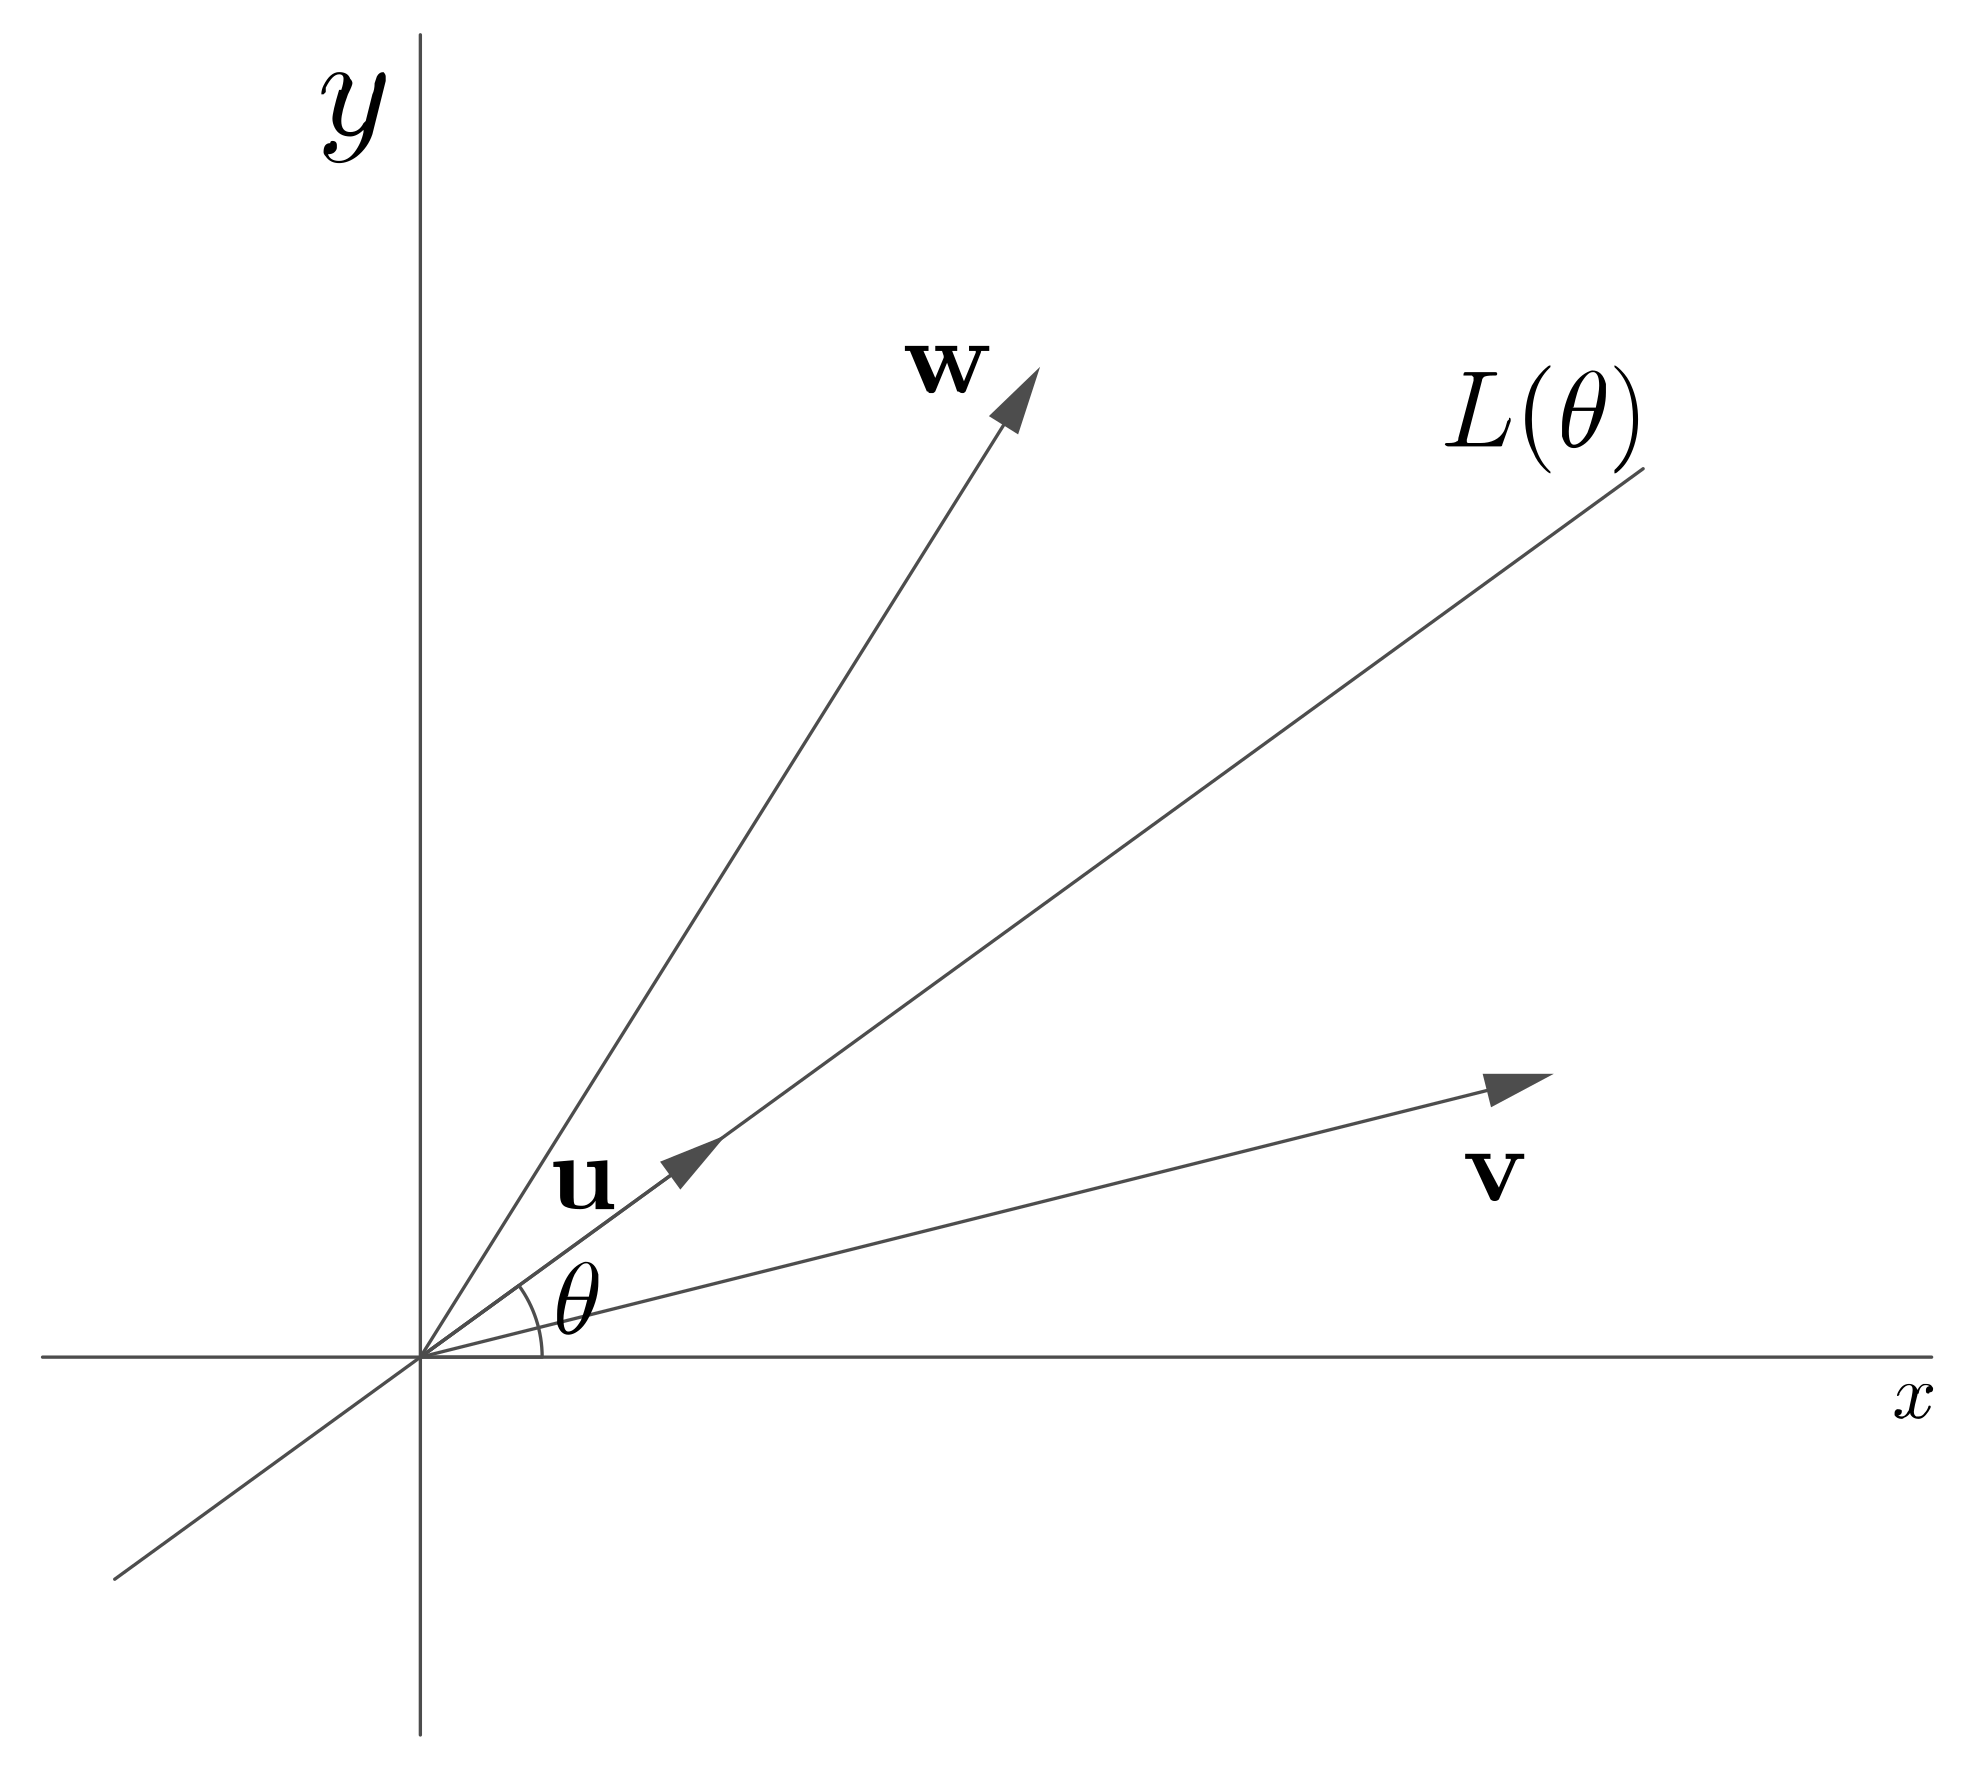
\includegraphics{Reflection.eps}} 
\caption{Reflecting across a line $L(\theta)$.}
\label{F:Reflection}
\end{center}
\end{figure}

\ba
\item Find a unit vector $\vu$ in the direction of the line $L(\theta)$. 

\item Let $\vv = \left[ \begin{array}{c} a\\b \end{array} \right]$ be an arbitrary vector in $\R^2$ as represented in Figure \ref{F:Reflection}. Determine the components of the vectors $\proj_{\vu} \vv$ and $\proj_{\perp \vu} \vv$. Reproduce Figure \ref{F:Reflection} and draw the vectors $\proj_{\vu} \vv$ and $\proj_{\perp \vu} \vv$ in your figure.

\item The vector labeled $\vw$ is the reflection of the vector $\vv$ across the line $L(\theta)$. Write $\vw$ in terms of $\vv$ and $\proj_{\vu} \vv$. Clearly explain your method.

\item Finally, show that the matrix $A$ such that $A \vv = \vw$ is given by 
\[A = \left[ \begin{array}{cr} \cos(2\theta)&\sin(2\theta) \\ \sin(2\theta)& -\cos(2\theta) \end{array} \right].\]
The matrix $A$ is the \emph{reflection} matrix across the line $L(\theta)$. (You will want to look up some appropriate trigonometric identities.)

\ea


\item In this exercise we will show that the only orthogonal $2 \times 2$ matrices are the rotation matrices $ \left[ \begin{array}{cr} \cos(\theta)&-\sin(\theta) \\ \sin(\theta)& \cos(\theta) \end{array} \right]$ and the reflection matrices $\left[ \begin{array}{cr} \cos(\theta)&\sin(\theta) \\ \sin(\theta) &-\cos(\theta) \end{array} \right]$ (see Exercise \ref{ex:Reflection_matrices}).  Throughout this exercise let $a$, $b$, $c$, and $d$  be real numbers such that $M = \left[ \begin{array}{cc} a&b \\ c&d \end{array} \right]$ is an orthogonal $2 \times 2$ matrix. Let $\vv_1= \left[ \begin{array}{c} a \\ c \end{array} \right]$ and $\vv_2= \left[ \begin{array}{c} b \\ d \end{array} \right]$ be the columns of $M$.

\ba

\item  Explain why the terminal point of $\vv_1$ in standard position lies on the unit circle. Then explain why there is an angle $\theta$ such that $a = \cos(\theta)$ and $c = \sin(\theta)$. What angle, specifically, is $\theta$? Draw a picture to illustrate. 

\item A similar argument to (b) shows that there is an angle $\alpha$ such that $\vv_2 = \left[ \begin{array}{c} b\\d \end{array} \right] = \left[ \begin{array}{c} \cos(\alpha)\\\sin(\alpha) \end{array} \right]$. Given that $M$ is an orthogonal matrix, how must $\alpha$ be related to $\theta$? Use this result to find the two possibilities for $\vv_2$ as a vector in terms of $\cos(\theta)$ and $\sin(\theta)$. (You will likely want to look up some trigonometric identities for this part of the problem.)

\item By considering the two possibilities from part (c), show that $M$ is either a rotation matrix or a reflection matrix. Conclude that the only $2 \times 2$ orthogonal matrices are the reflection and rotation matrices. 

\ea 
	

\item Suppose $A, B$ are orthogonal matrices of the same size. 
  \ba 
	\item Show that $AB$ is also an orthogonal matrix.
	\item Show that $A^\tr$ is also an orthogonal matrix.
	\item Show that $A^{-1}$ is also an orthogonal matrix.
	\ea
	
\item Label each of the following statements as True or False. Provide justification for your response.
	\ba
	\item \textbf{True/False} Any orthogonal subset of $\R^n$ is linearly independent.
	\item \textbf{True/False} Every single vector set is an orthogonal set.
	\item \textbf{True/False} If $S$ is an orthogonal set in $\R^n$ with exactly $n$ nonzero vectors, then $S$ is a basis for $\R^n$.  
	\item \textbf{True/False} Every set of three linearly independent vectors in $\R^3$ is an orthogonal set.
%	\item \textbf{True/False} If $A$ is an $n \times n$ orthogonal matrix, then $A^{\tr}$ must also be an orthogonal matrix. 
%	\item \textbf{True/False} If $A$ is an $n \times n$ orthogonal matrix, then $A^{-1}$ must also be an orthogonal matrix.
	\item \textbf{True/False} If $A$ and $B$ are $n \times n$ orthogonal matrices, then $A+B$ must also be an orthogonal matrix.
%	\item \textbf{True/False} If $A$ and $B$ are $n \times n$ orthogonal matrices, then $AB$ must also be an orthogonal matrix.
	\item \textbf{True/False} If the set $S=\{\vv_1, \vv_2, \ldots, \vv_n\}$ is an orthogonal set in $\R^n$, then so is the set $\{c_1\vv_1, c_2\vv_2, \ldots, c_n\vv_n\}$ for any scalars $c_1$, $c_2$, $\ldots$, $c_n$.
	\item \textbf{True/False} If $\CB=\{\vv_1, \vv_2, \ldots, \vv_n\}$ is an orthogonal basis of $\R^n$, then so is $\{c_1\vv_1$, $c_2\vv_2$, $\ldots$, $c_n\vv_n\}$ for any nonzero scalars $c_1$, $c_2$, $\ldots$, $c_n$.
	\item \textbf{True/False} If $A$ is an $n\times n$ orthogonal matrix, the rows of $A$ form an orthonormal basis of $\R^n$.
	\item \textbf{True/False} If $A$ is an orthogonal matrix, any matrix obtained by interchanging columns of $A$ is also an orthogonal matrix.
	\ea
	
\ee

\csection{Project: Understanding Rotations in 3-Space}
\label{sec:proj_3d_rotate}

Recall that a counterclockwise rotation of $2$-space around the origin by an angle $\theta$ is accomplished by left multiplication by the matrix $\left[ \begin{array}{cr} \cos(\theta)&-\sin(\theta) \\ \sin(\theta)&\cos(\theta) \end{array} \right]$. Notice that the columns of this rotation matrix are orthonormal, so this rotation matrix is an orthogonal matrix. As the next activity shows, rotation matrices in 3D are also orthogonal matrices.

\begin{pactivity} \label{act:rot_det} Let $R$ be a rotation matrix in 3D.  A rotation does not change lengths of vectors, nor does it change angles between vectors. Let $\ve_1 = [ 1 \ 0 \ 0]^{\tr}$, $\ve_2 = [0 \ 1 \ 0]^{\tr}$, and $\ve_3 = [0 \ 0 \ 1]^{\tr}$ be the standard unit vectors in $\R^3$.
\ba
\item Explain why the columns of $R$ form an orthonormal set. (Hint: How are $R \ve_1$, $R\ve_2$, and $R\ve_3$ related to the columns of $R$?) 

\item Explain why $R$ is an orthogonal matrix. What must be true about $\det(R)$? (Hint: What is $R^{\tr}$ and what is $\det(R^{\tr}R)$?)

\ea

\end{pactivity}

By Project Activity \ref{act:rot_det} we know that the determinant of any rotation matrix is either $1$ or $-1$. Having a determinant of $1$ preserves orientation, and we will identify these rotations as being counterclockwise, and we will identify the others with determinant of $-1$ as being clockwise. We will set the convention that a rotation is always measured counterclockwise (as we did in $\R^2$), and so every rotation matrix will have determinant $1$. 

Returning to the counterclockwise rotation of $2$-space around the origin by an angle $\theta$ determined by left multiplication by the matrix $\left[ \begin{array}{cr} \cos(\theta)&-\sin(\theta) \\ \sin(\theta)&\cos(\theta) \end{array} \right]$, we can think of this rotation in $3$-space as the rotation that keeps points in the $xy$ plane in the $xy$ plane, but rotates these points counterclockwise around the $z$ axis. In other words, in the standard $xyz$ coordinate system, with standard basis $\ve_1$, $\ve_2$, $\ve_3$, our rotation matrix $R$ has the property that $R \ve_3 = \ve_3$. Now $R \ve_3$ is the third column of $R$, so the third column of $R$ is $\ve_3$. Similarly, $R \ve_1$ is the first column of $R$ and $R \ve_2$ is the second column of $R$. Since $R$ is a counterclockwise rotation of the $xy$ plane space around the origin by an angle $\theta$ it follows that this rotation is given by the matrix
\begin{equation} \label{eq:rot_z}
R_{\ve_3}(\theta) = \left[ \begin{array}{ccc} \cos(\theta)&-\sin(\theta)&0 \\ \sin(\theta)&\cos(\theta)&0 \\ 0&0&1 \end{array} \right].
\end{equation}

In this notation in (\ref{eq:rot_z}), the subscript gives the direction of the line fixed by the rotation and the angle provides the counterclockwise rotation in the plane perpendicular to this vector. This vector is called a \emph{normal} vector for the rotation. Note also that the columns of $R_{\ve_3}(\theta)$ form an orthogonal set such that each column vector has norm $1$. 

This idea describes a general rotation matrix $R_{\vn}(\theta)$ in 3D by specifying a normal vector $\vn$ and an angle $\theta$. For example, with roll, a normal vector points from the tail of the aircraft to its tip. It is our goal to understand how we can determine an arbitrary rotation matrix of the form $R_{\vn}(\theta)$. We can accomplish this by using the rotation around the $z$ axis and change of basis matrices to find rotation matrices around other axes. Let $\CS = \{\ve_1, \ve_2, \ve_3\}$ be the standard basis for $\R^3$

\begin{pactivity} \label{act:rot_x} In this activity we see how to determine the rotation matrix around the $x$ axis using the matrix $R_{\ve_3}(\theta)$ and a change of basis.
\ba
\item  Define a new ordered basis $\CB$ so that our axis of rotation is the third vector. So in this case the third vector in $\CB$ will be $\ve_1$. The other two vectors need to make $\CB$ an orthonormal set. So we have plenty of choices. For example, we could set $\CB = \{\ve_2, \ve_3, \ve_1\}$. Find the change of basis matrix $\underset{\CS \leftarrow \CB}{P}$ from $\CB$ to $\CS$.
	
\item Use the change of basis matrix from part (a) to find the change of basis matrix $\underset{\CB \leftarrow \CS}{P}$ from $\CS$ to $\CB$.

\item To find our rotation matrix around the $x$ axis, we can first change basis from $\CS$ to $\CB$, then perform a rotation around the new $z$ axis using (\ref{eq:rot_z}), then changing basis back from $\CB$ to $\CS$. In other words, 
\[R_{\ve_1}(\theta) = \underset{\CS \leftarrow \CB}{P} R_{\ve_3}(\theta) \underset{\CB \leftarrow \CS}{P}.\]
Find the entries of this matrix $R_{\ve_1}(\theta)$.

\ea

\end{pactivity}


\noindent \textbf{IMPORTANT NOTE:} We could have considered using $\CB_1 = \{\ve_3, \ve_2, \ve_1\}$ in Project Activity \ref{act:rot_x} instead of $\CB = \{\ve_2, \ve_3, \ve_1\}$. Then we would have 
\[\underset{\CS \leftarrow \CB_1}{P} = \left[ \begin{array}{ccc} 0&0&1 \\ 0&1&0 \\ 1&0&0 \end{array} \right].\]
The difference between the two options is that, in the first we have $\det\left(\underset{\CS \leftarrow \CB_1}{P}\right) = -1$ while $\det\left(\underset{\CS \leftarrow \CB}{P} \right) = 1$ in the second. Using $\CB_1$ will give clockwise rotations while $\CB$ gives counterclockwise rotations (this is the difference between a left hand system and a right hand system). So it is important to ensure that our change of basis matrix is one with determinant $1$. 

\begin{pactivity} \label{act:rot_y} Repeat Project Activity \ref{act:rot_y} to find the 3D rotation around the $y$ axis. 

\end{pactivity}

We do one more example to illustrate the process before tackling the general case. 

\begin{pactivity} \label{act:rot_ex} In this activity we find the rotation around the axis given by the line $x=y/2=z$. This line is in the direction of the vector $\vn = [1 \ 2 \ 1]^{\tr}$. So we start with making a unit vector in the direction of $\vn$ as the third vector in an ordered basis $\CB$. The other two vectors need to make $\CB$ an orthonormal set with $\det\left(\underset{\CS \leftarrow \CB}{P} \right) = 1$.
\ba
\item  Find a unit vector $\vw$ in the direction of $\vn$. 
	
	
\item Show that $[2 \ -1 \ 0]^{\tr}$ is orthogonal to the vector $\vw$ from part (a). Then find a unit vector $\vv$ that is in the same direction as $[2 \ -1 \ 0]^{\tr}$. 


\item Let $\vv$ be as in the previous part. Now the trick is to find a third unit vector $\vu$ so that $\CB = \{\vu, \vv, \vw\}$ is an orthonormal set. This can be done with the cross product. If $\va = [a_1 \ a_2 \ a_3]^{\tr}$ and $\vb = [b_1 \ b_2 \ b_3]^{\tr}$, then the cross product $\va \times \vb$ of $\va$ and $\vb$ is the vector 
\[\va \times \vb = \left(a_2b_3-a_3b_2\right) \ve_1 - \left(a_1b_3-a_3b_1\right) \ve_2 + \left(a_1b_2-a_2b_1\right) \ve_3.\]
(You can check that $\{\va \times \vb, \va, \vb\}$ is an orthogonal set that gives the correct determinant for the change of basis matrix.) Use the cross product to find a unit vector $\vu$ so that $\CB = \{\vu, \vv, \vw\}$ is an orthonormal set. 
 

\item Find the entries of the matrix $R_{\vw}(\theta)$. 

\ea

\end{pactivity}

In the next activity we summarize the general process to find a 3D rotation matrix $R_{\vn}(\theta)$ for any normal vector $\vn$. There is a GeoGebra applet at \url{https://www.geogebra.org/m/n9gbjhfx} that allows you to visualize rotation matrices in 3D. 

\begin{pactivity} \label{act:rot_general} Let $\vn = [n_1 \ n_2 \ n_3]^{\tr}$ be a normal vector (nonzero) for our rotation. We need to create an orthonormal basis $\CB = \{\vu, \vv, \vw\}$ where $\vw$ is a unit vector in the direction of $\vn$ so that the change of basis matrix $\underset{\CS \leftarrow \CB}{P}$ has determinant $1$. 
\ba
\item Find, by inspection, a vector $\vy$ that is orthogonal to $\vn$. (Hint: You may need to consider some cases to ensure that $\vv$ is not the zero vector.) 


\item Once we have a normal vector $\vn$ and a vector $\vy$ orthogonal to $\vn$, the vector $\vz = \vy \times \vn$ gives us an orthogonal set $\{\vz, \vy, \vn\}$. We then normalize each vector to create our orthonormal basis $\CB = \{\vu, \vv, \vw\}$. Use this process to find the matrix that produces a $45^{\circ}$ counterclockwise rotation around the normal vector $[1 \ 0 \ -1]^{\tr}$. 

\ea

\end{pactivity}
